\documentclass{beamer}

 
\usetheme{Madrid}
\usepackage{natbib}
\bibliographystyle{apalike}
% make bibliography entries smaller
\renewcommand\bibfont{\scriptsize}
% If you have more than one page of references, you want to tell beamer
% to put the continuation section label from the second slide onwards
\setbeamertemplate{frametitle continuation}[from second]
% Now get rid of all the colours
\setbeamercolor*{bibliography entry title}{fg=black}
\setbeamercolor*{bibliography entry author}{fg=black}
\setbeamercolor*{bibliography entry location}{fg=black}
\setbeamercolor*{bibliography entry note}{fg=black}
% and kill the abominable icon
\setbeamertemplate{bibliography item}{}
\newlength{\sepmargin}
\newlength{\sepwid}
\newlength{\onecolwid}
\newlength{\twocolwid}
\newlength{\threecolwid}
% The following measures are used for 2 columns
\setlength{\sepmargin}{0.055\paperwidth} % Separation width (white space) between columns
\setlength{\sepwid}{0.03\paperwidth} % Separation width (white space) between columns
\setlength{\onecolwid}{0.43\paperwidth} % Width of one column
\setlength{\twocolwid}{0.9\paperwidth} % Width of two columns
\usepackage{multicol}
\usepackage{subfig}
 
%----------------------------------------------------------------------------------------
%	TITLE PAGE
%----------------------------------------------------------------------------------------

\title[Corporate Governance and Performance]{The Relationship Between Corporate Governance and Company Performance \\~\\ \small {New Factors, New Models, New Approaches to Causality} } % The short title appears at the bottom of every slide, the full title is only on the title page

\author{Conor Reid} % Your name
\institute [UCD Smurfit School] % Your institution as it will appear on the bottom of every slide, may be shorthand to save space
{
Dr. James McDermott \& Dr. Miguel Nicolau \\
\medskip
UCD Michael Smurfit Graduate Business School \\
\medskip
\textit{conor.reid@ucdconnect.ie} % Your email address
}

\date{\today} % Date, can be changed to a custom date

\begin{document}

\begin{frame}
\titlepage % Print the title page as the first slide
\end{frame}

\begin{frame}
\frametitle{Overview} % Table of contents slide, comment this block out to remove it
\tableofcontents % Throughout your presentation, if you choose to use \section{} and \subsection{} commands, these will automatically be printed on this slide as an overview of your presentation
\end{frame}

%Put the logo on every page
\pgfdeclareimage[height=1.3cm]{logo}{images/logo.png}
\logo{\pgfuseimage{logo}\hspace*{0.5cm}}


\section{Motivation and Previous Work}
\begin{frame}[t]
\frametitle{Motivation and Previous Work}
{Corporate governance models vary widely across firms, and there is much debate on the impact of these differing styles on company performance.}
\begin{itemize}
\item {How can these features be optimised for best performance? }
\item {What defines {\it best performance}?}
\end{itemize}

\vspace{1cm}

{\cite{moldovan2015learning} attempted to answer these questions. They:}
\begin{itemize}
\item {Acquired data from the Bloomberg financial data repository.}
\item {Tobins Q Score and Altman Z Score for success.}
\item {Worked to learn explanatory and predictive models.}
\item {Proposed rules for success. }
\end{itemize}

\end{frame}

\begin{frame}
\frametitle{Motivation and Previous Work}
\cite{moldovan2015learning}: 
\begin{itemize}
\item[$\checkmark$] Identified a number of correlations across multiple algorithms and measures. \\
\item [$\times$] Thresholded on continuous dependent variables. \\
\item [$\times$] Unexplored algorithms and techniques. \\
\item [$\times$] Correlation $\neq$ Causation.
\end{itemize}
\vspace{0.5cm}
Other Work
\begin{itemize}
\item[$\blacksquare$] \cite{holland1986statistics} discusses statistical models for causal inference. \\
\item [$\blacksquare$] \cite{pearl1995theory}, \cite{pearl2009causality} discuss causality extensively.
\end{itemize}
\end{frame}


%------------------------------------------------ 
\section{Approach}
\begin{frame}[t]
\frametitle{Approach}
My Approach \\~\\
\begin{enumerate}
\item [$\blacksquare$]  Reproduce some results of \cite{moldovan2015learning}. \\~\\
\item [$\blacksquare$]  Integrate auxiliary independant and dependent covariates, e.g: 
	\indent
	\begin{itemize} 
		\item [\footnotesize {Ind}] 		CEO compensation
		\item [\footnotesize {Ind}]		Environmental \& social impact disclosure
		\item [\footnotesize {Dep}]		Beneish M-Score  \\~\\ 
	\end{itemize}
\item [$\blacksquare$]  Apply modern causal research.
\end{enumerate}

\end{frame}
%------------------------------------------------
\section {Methods}
\begin{frame}[t]
\frametitle{Methods}
My Methods
\begin{enumerate}
\item [$\blacksquare$]  Reproduce : \\Using the same data, implement {\texttt Adaboost} and \texttt{J48} [ \texttt{C5.0} ], as well as \texttt{Regularised Linear Regression}. \\~\\
\item [$\blacksquare$]  Auxiliary Features : \\ Use Bloomberg repository to extract, merge using {\texttt R}. \\~\\
\item [$\blacksquare$]  Causal Research : \\ Using modified data, implement \texttt{Propensity Score Matching}.  \\~\\
\end{enumerate}
\end{frame}
%------------------------------------------------
\section {Results}
\begin{frame}[t]
\frametitle{Results - CEO Compensation}
\begin{tabular}{ll}
{\bf Dataset} & S\&P 500  \\
{\bf Dependent Variable} & Tobins Q Score \\
{\bf Treatment} & CEO Comp $>$ median(CEO Comp)? 1 : 0  \\
{\bf Estimate ($\% \Delta $)} &  (-0.06 $\sim$ -0.11) \\~\\
{\bf Matching Plots} &
\end{tabular}
\vspace{-0.8cm}
\begin{figure}[h!]
\centering
\footnotesize{\subfloat[\footnotesize{Asset}]{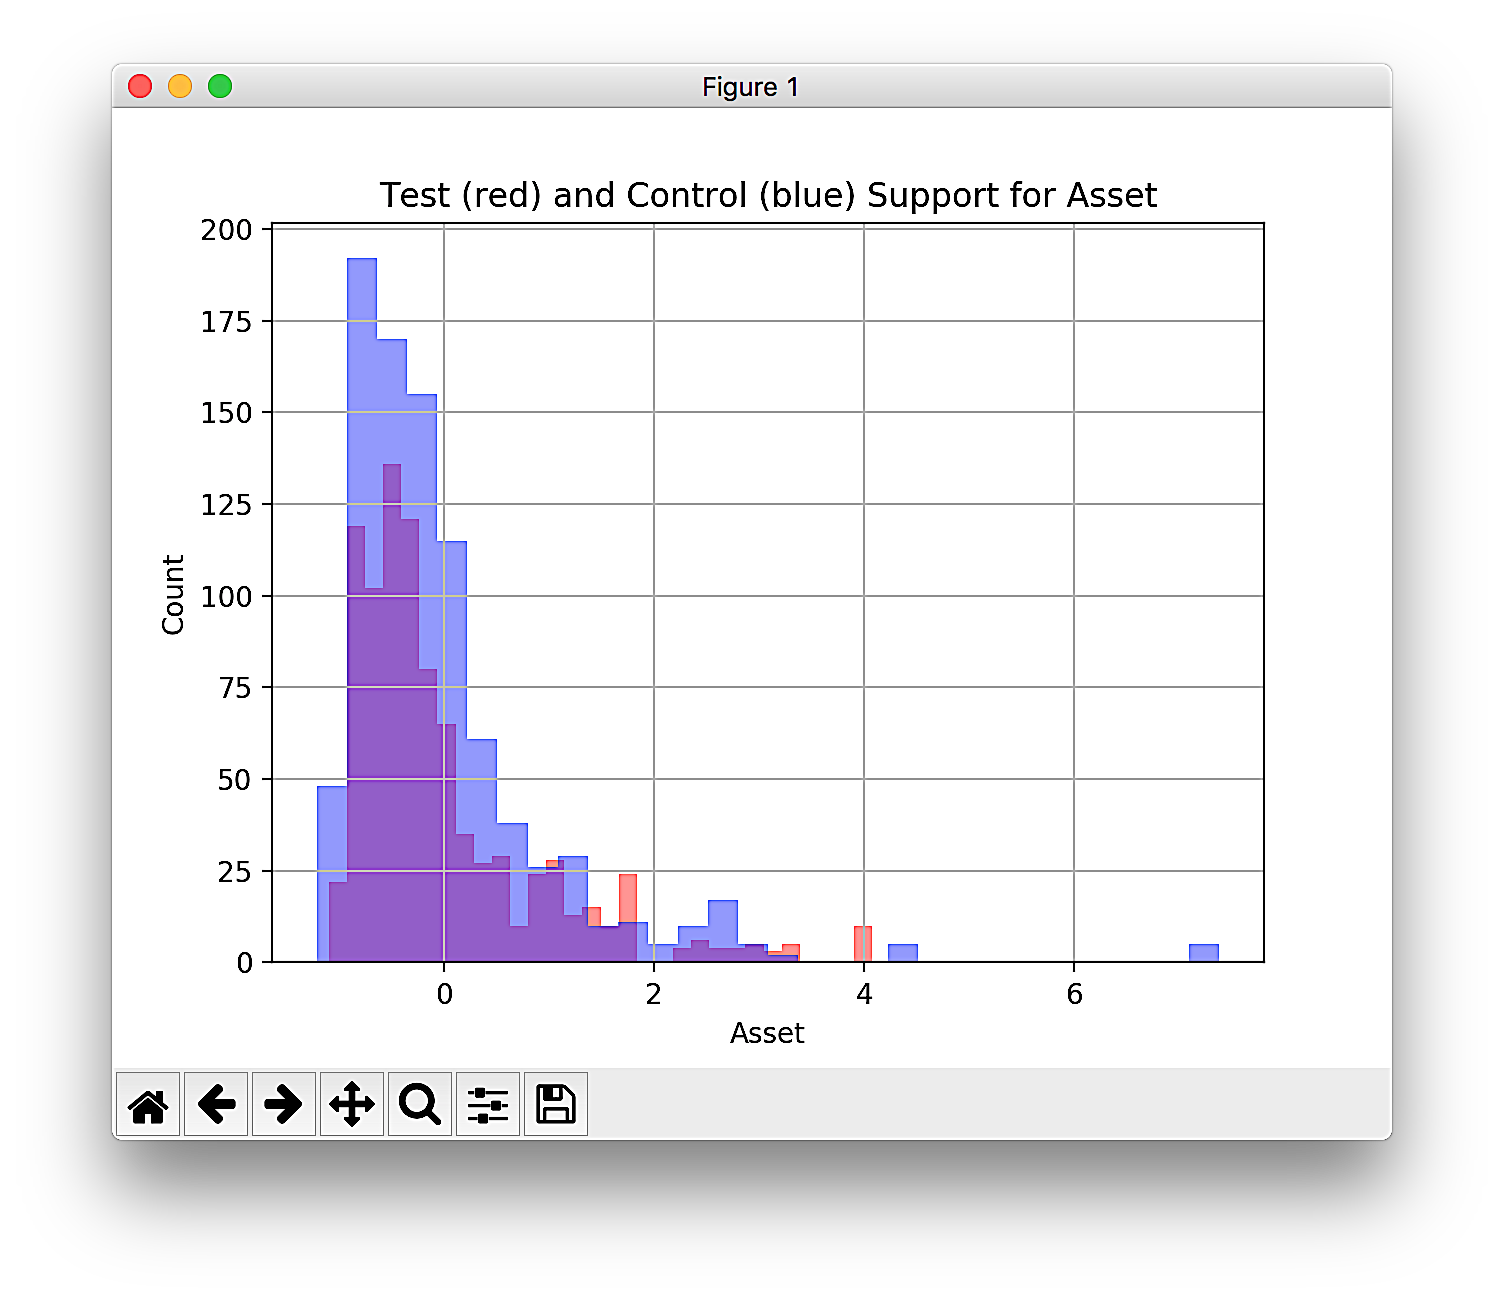
\includegraphics[width = 1.5in]{images/causal/CEOPayOverMedian/tobin/Asset.png}}}
\footnotesize{\subfloat[\footnotesize{EBITDA 12Mth}]{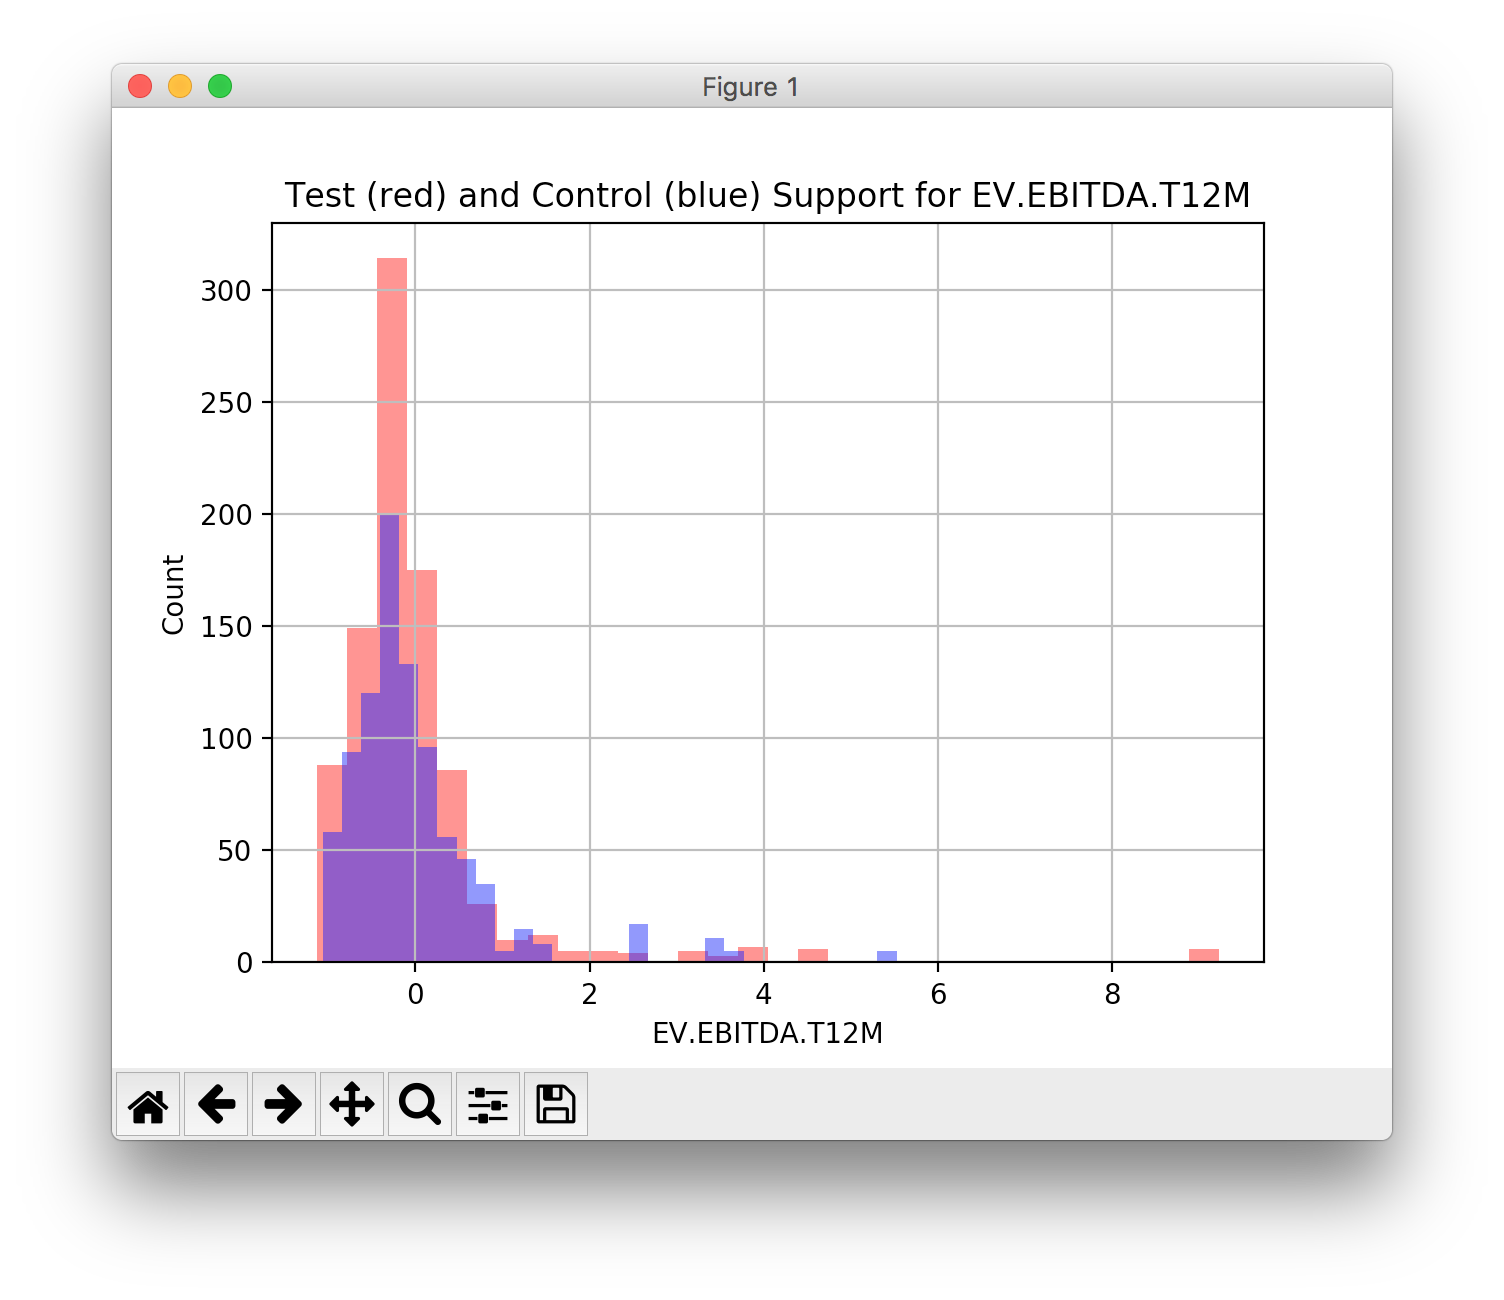
\includegraphics[width = 1.5in]{images/causal/CEOPayOverMedian/tobin/EV_EBITDA_T12M.png}} }
\footnotesize{\subfloat[\footnotesize{ROC}]{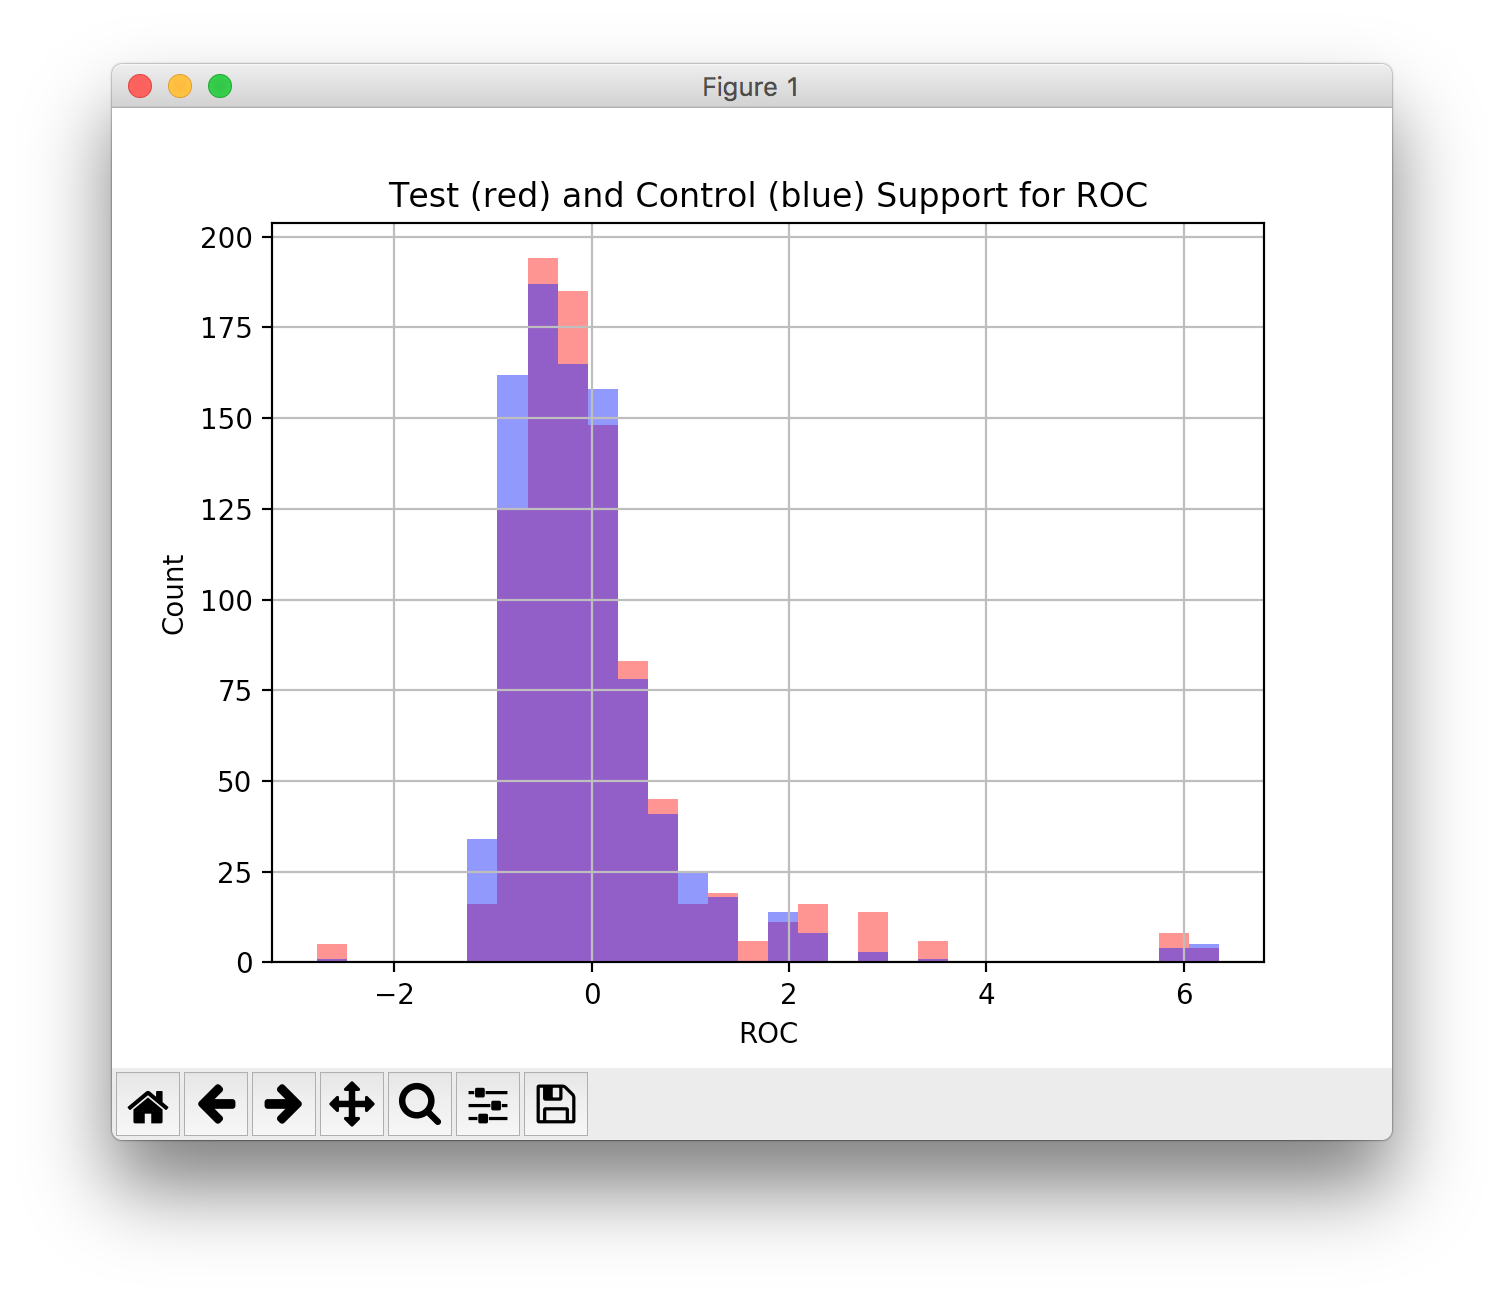
\includegraphics[width = 1.5in]{images/causal/CEOPayOverMedian/tobin/ROC.png}} }
\end{figure}
\end{frame}
%------------------------------------------------
\begin{frame}[t]
\frametitle{Results -  Indep Lead Director and Financial Leverage}
\begin{tabular}{ll}
{\bf Dataset} & STOXX Europe 600  \\
{\bf Dependent Variable} & Altman Z Score  \\
{\bf Treatment} & \footnotesize{(Indep Lead Dir \& Financial Leverage $>$ 2.5)? 1 : 0 } \\
{\bf Estimate ($\% \Delta $)} & (-0.24 $\sim$ -0.30)  \\~\\
{\bf Matching Plots} &
\end{tabular}
\vspace{-0.8cm}
\begin{figure}[h!]
\centering
\footnotesize{\subfloat[\footnotesize{Asset}]{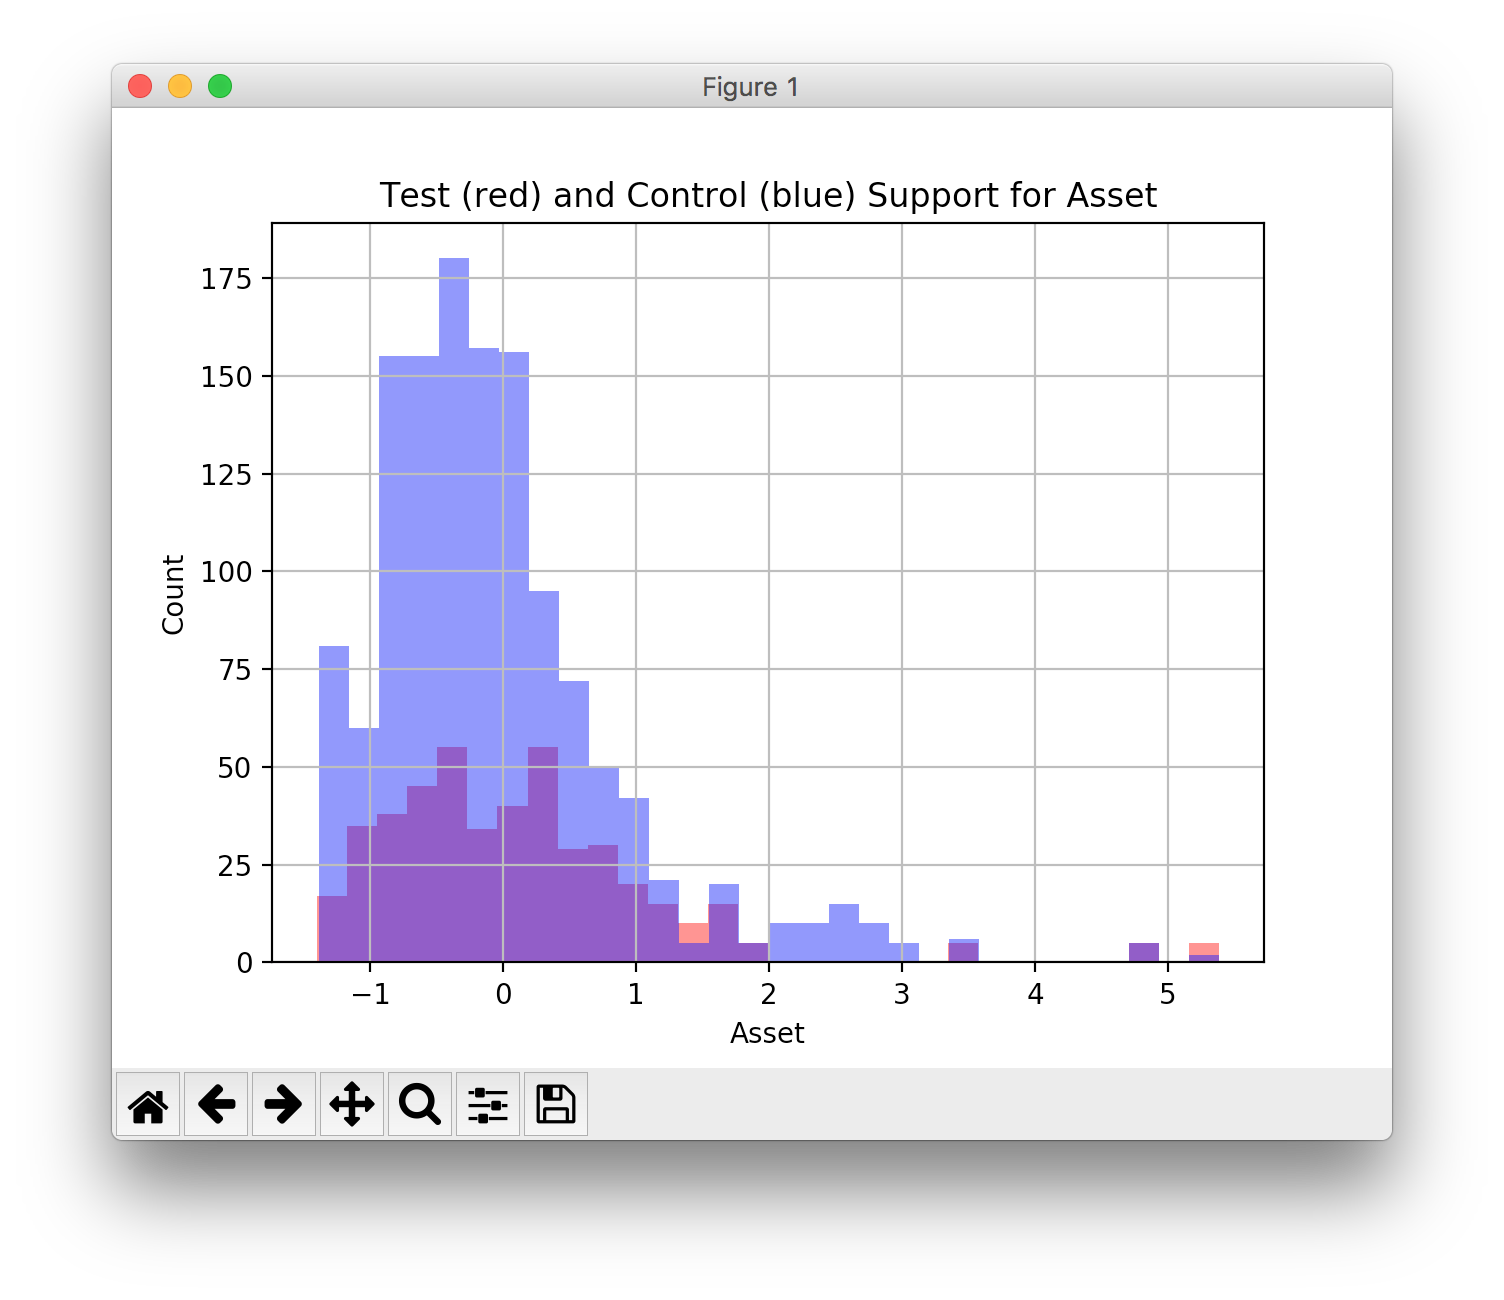
\includegraphics[width = 1.5in]{images/causal/indepDirFinlL/altman/Asset.png}}}
\footnotesize{\subfloat[\footnotesize{P/B}]{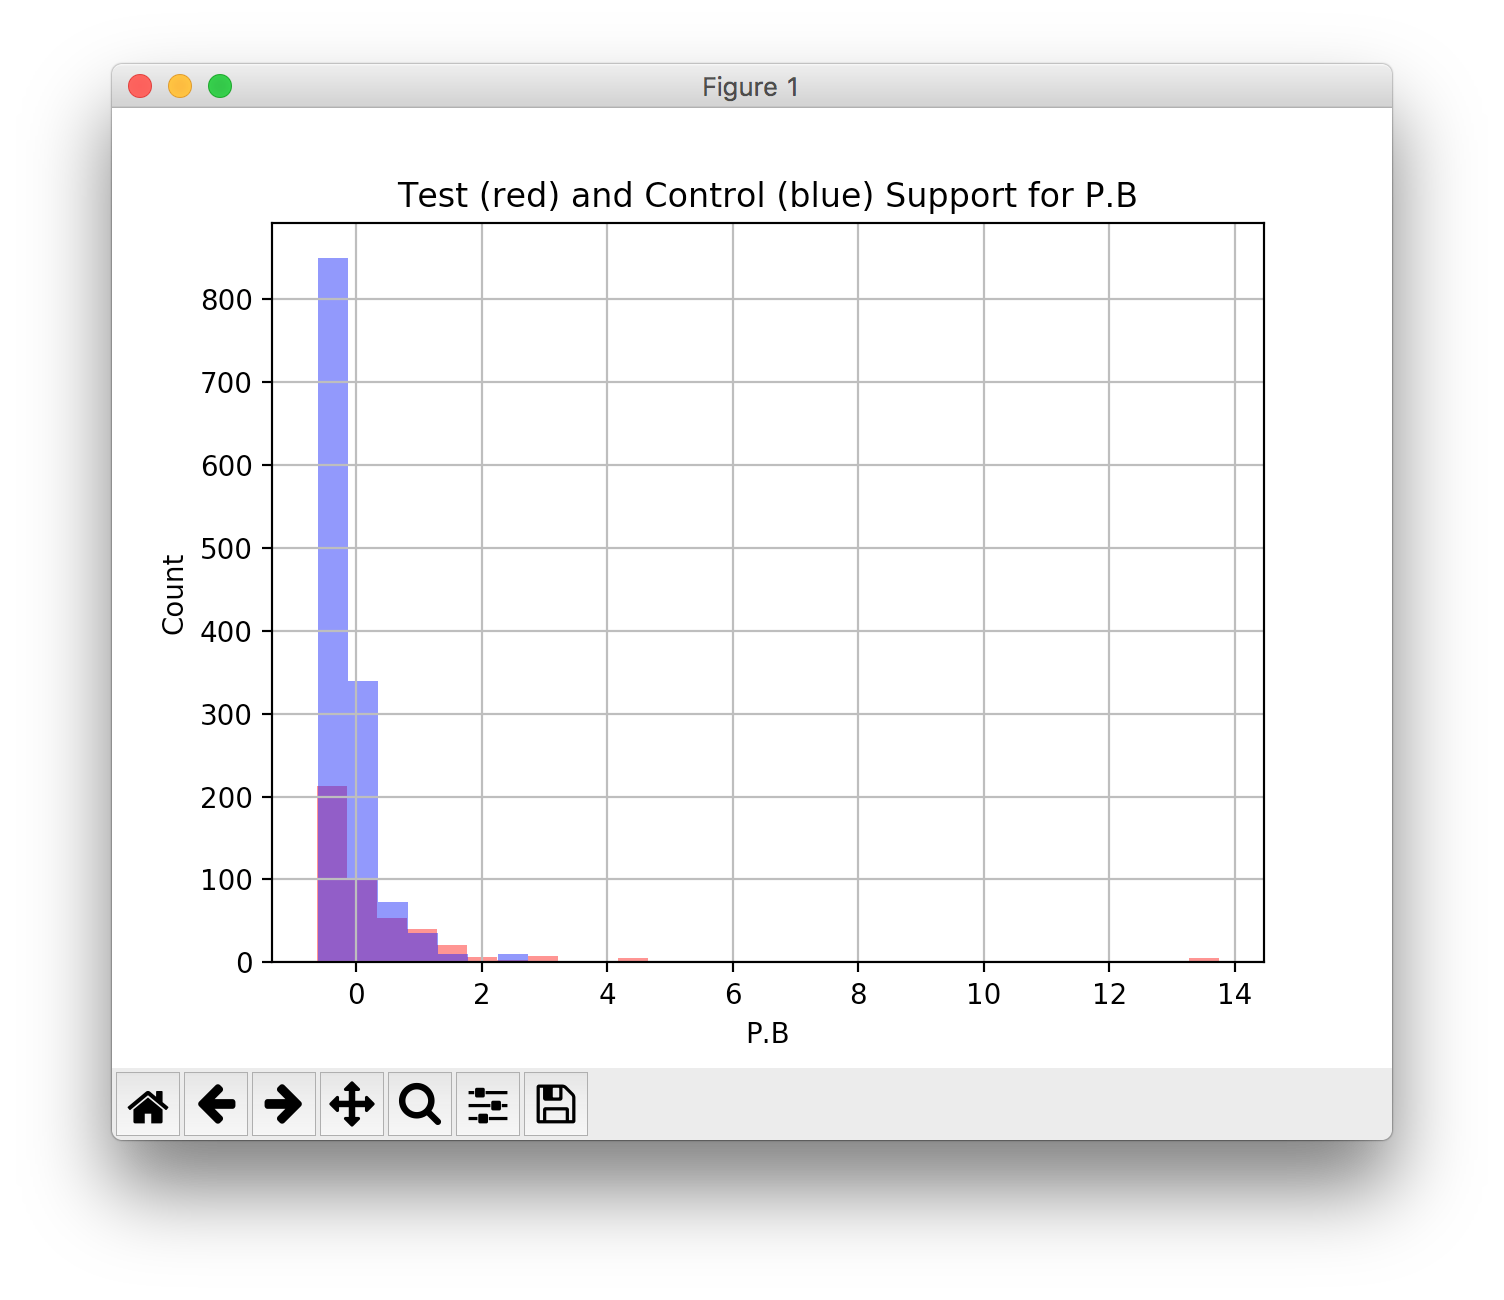
\includegraphics[width = 1.5in]{images/causal/indepDirFinlL/altman/PB.png}} }
\footnotesize{\subfloat[\footnotesize{EBITDA}]{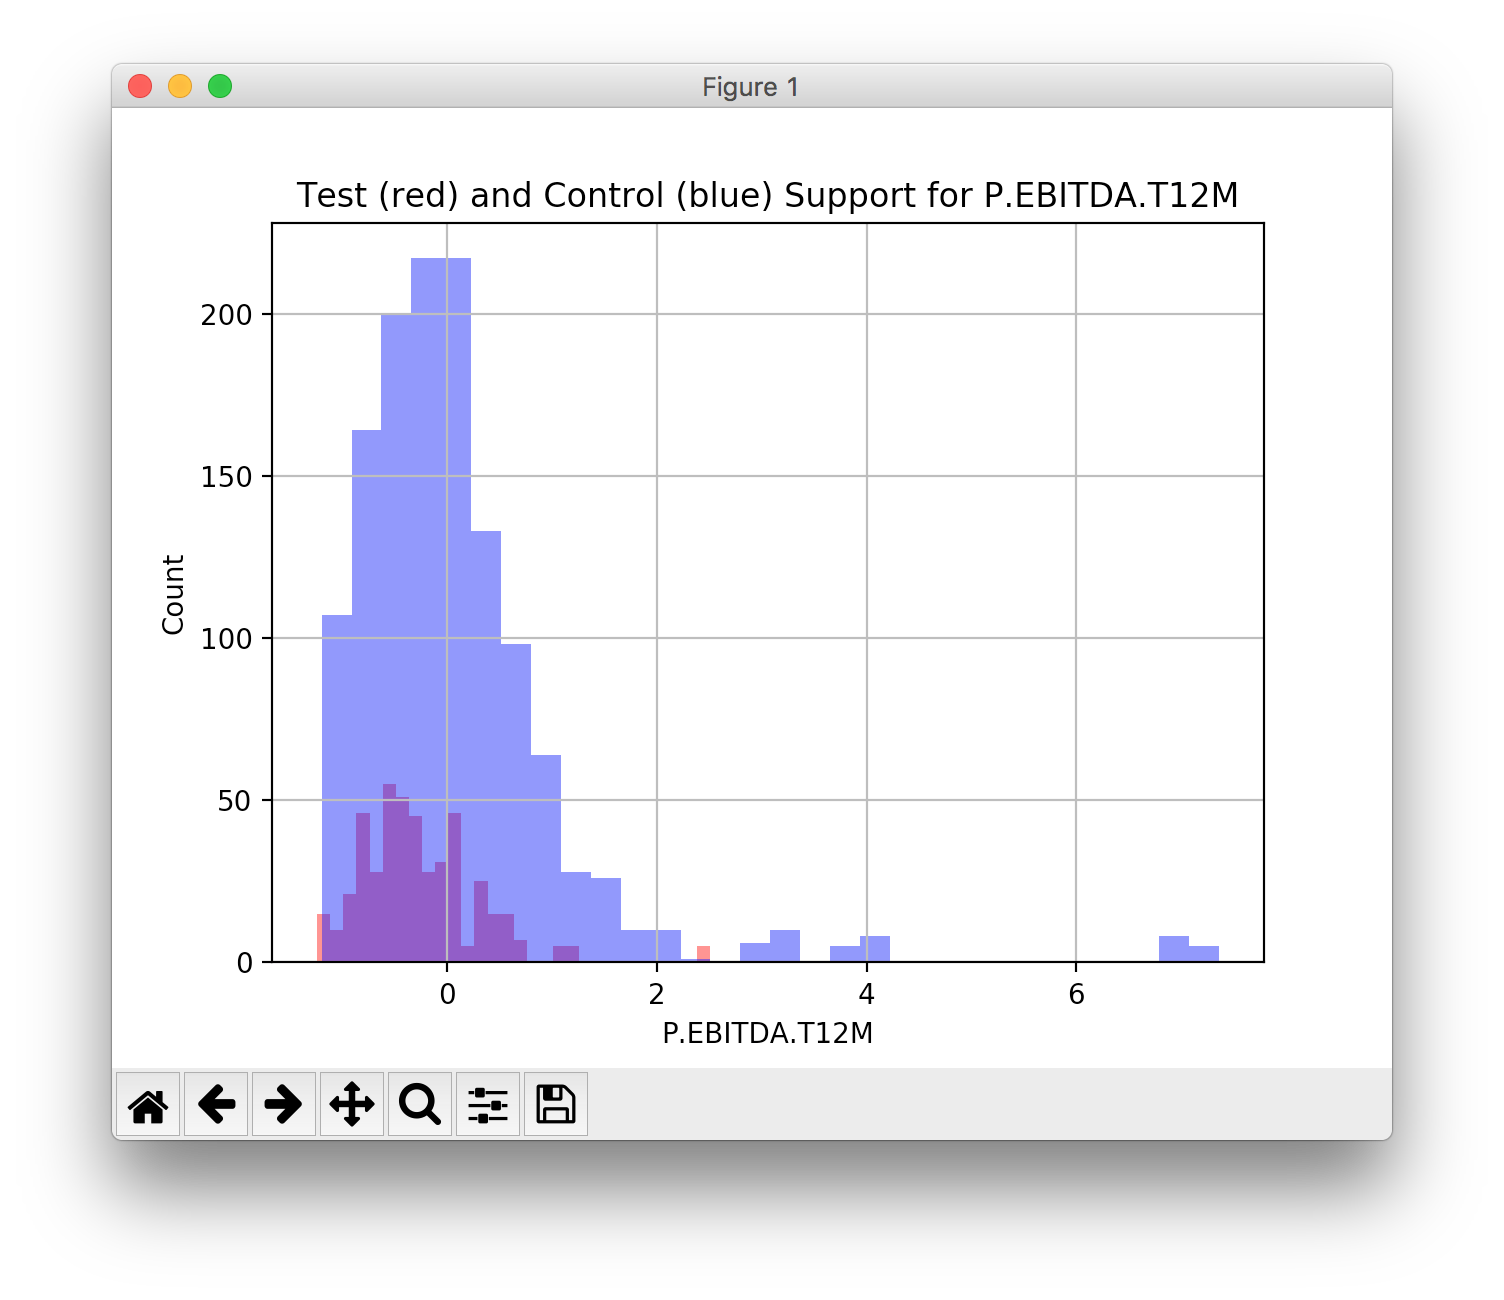
\includegraphics[width = 1.5in]{images/causal/indepDirFinlL/altman/P_EBITDA_T12M.png}} }
\end{figure}
\end{frame}
%------------------------------------------------
%\begin{frame}[t]
%\frametitle{Results - Indep Chairman or Female CEO}
%\begin{tabular}{ll}
%{\bf Dataset} & STOXX Europe 600  \\
%{\bf Dependent Variable} & Tobins Q Score  \\
%{\bf Treatment} & {(Indep Chairman $\mid$  Female CEO)? 1 : 0 } \\
%{\bf Estimate ($\% \Delta $)} & (0.07 $\sim$ 0.13) \\~\\
%{\bf Matching Plots} &
%\end{tabular}
%\vspace{-0.8cm}
%\begin{figure}[h!]
%\centering
%\footnotesize{\subfloat[\footnotesize{Asset}]{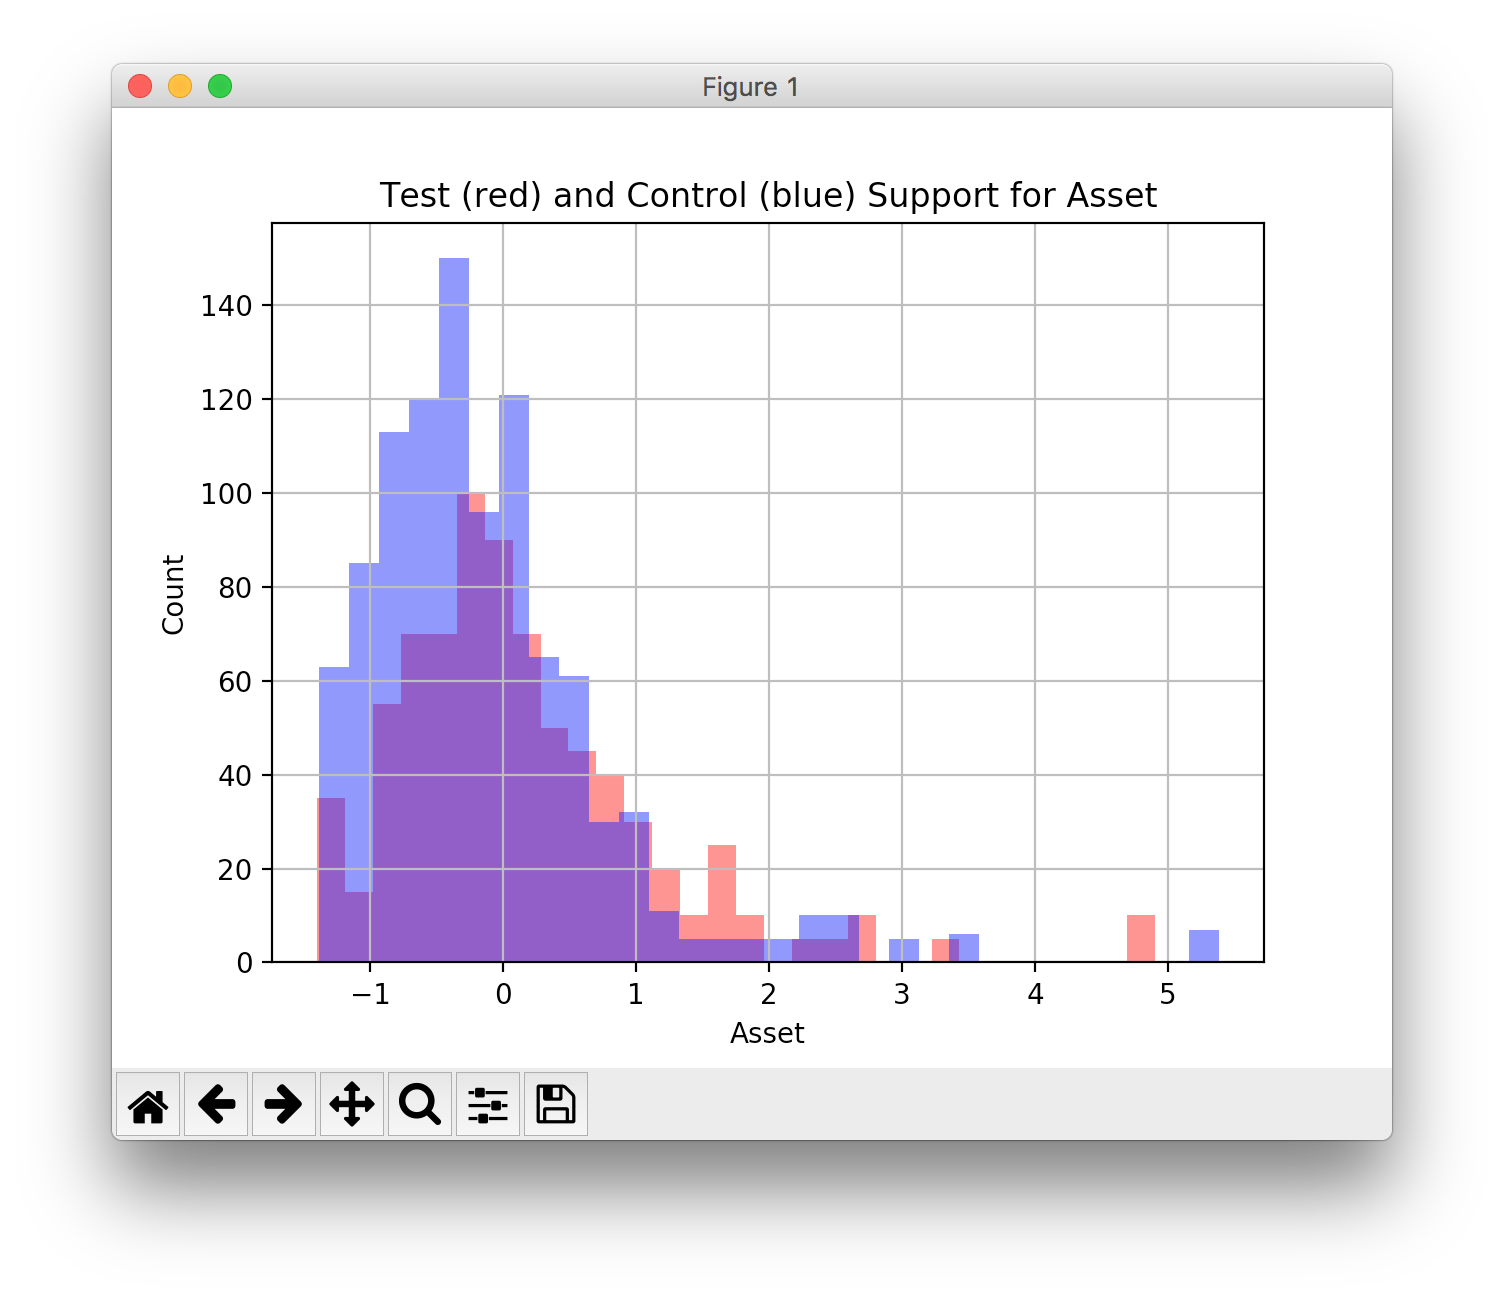
\includegraphics[width = 1.5in]{images/causal/Indep_Chrprsn_Feml_CEO_or_Equiv/tobin/Asset.png}}}
%\footnotesize{\subfloat[\footnotesize{OPM}]{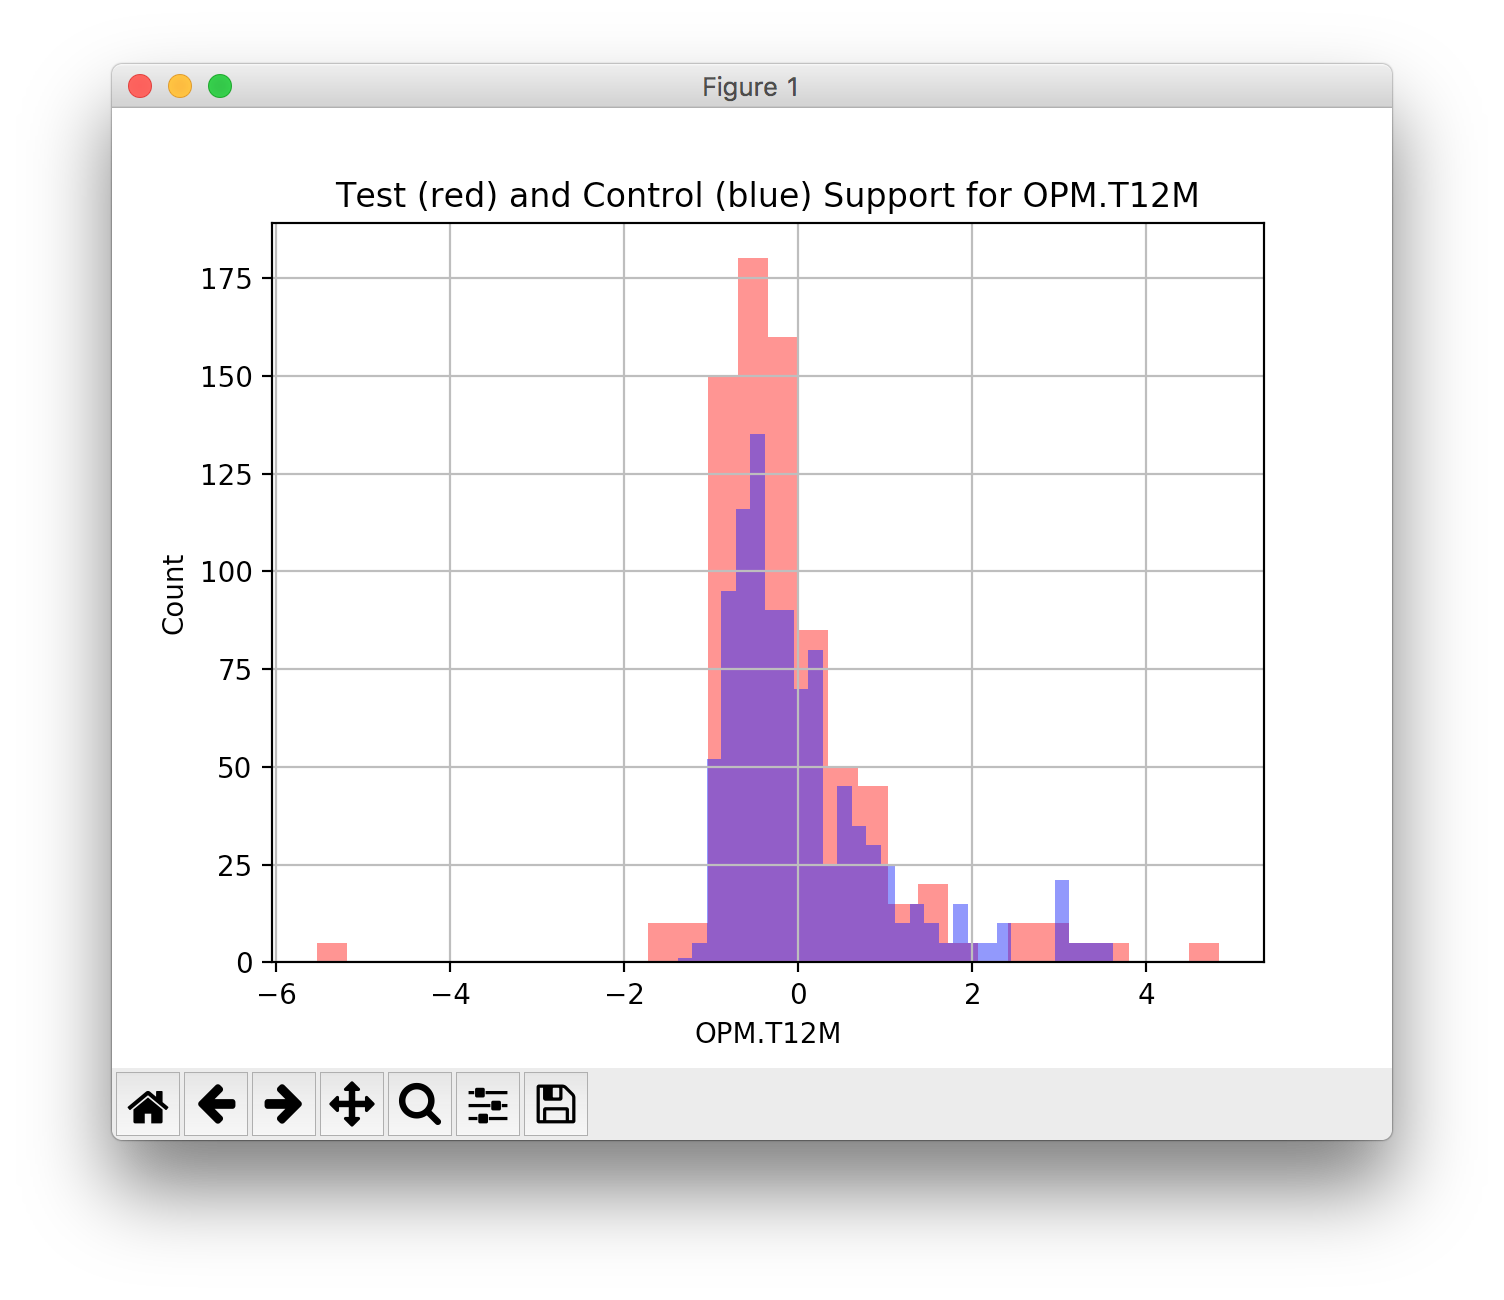
\includegraphics[width = 1.5in]{images/causal/Indep_Chrprsn_Feml_CEO_or_Equiv/tobin/OPM_T12M.png}} }
%\footnotesize{\subfloat[\footnotesize{Adj ROE}]{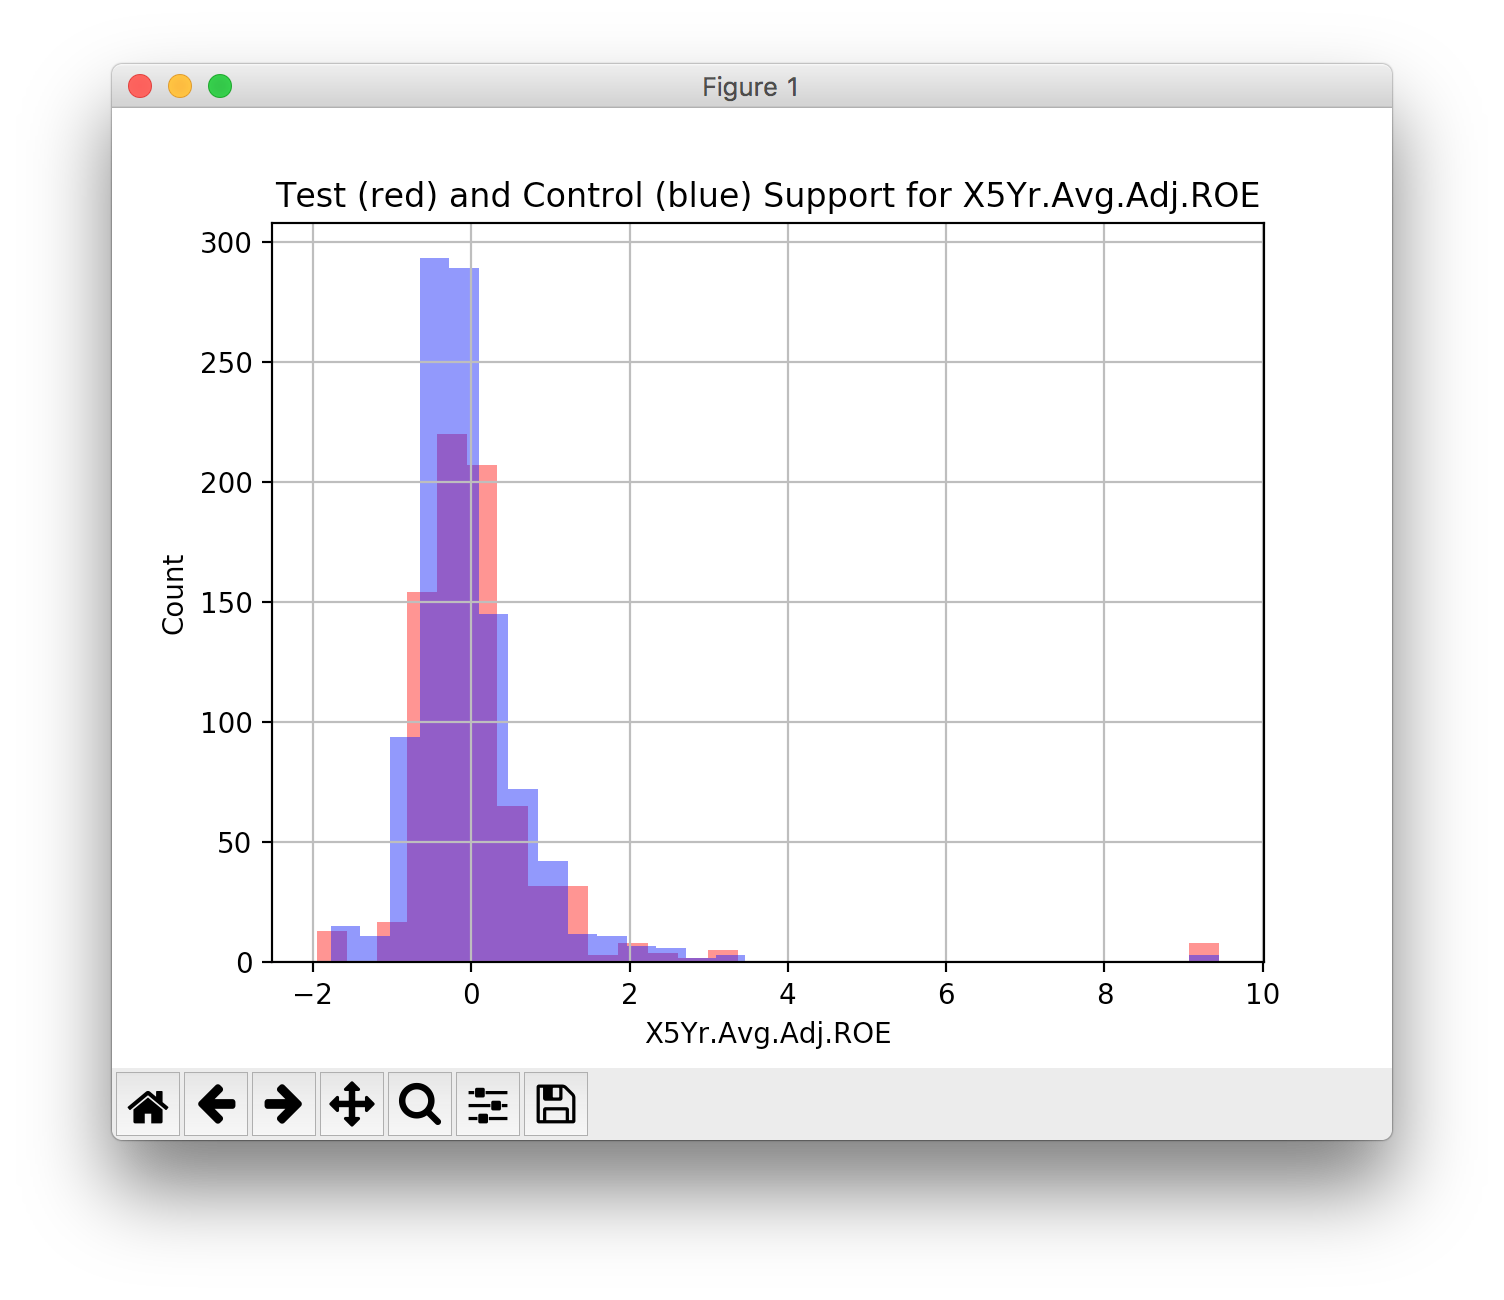
\includegraphics[width = 1.5in]{images/causal/Indep_Chrprsn_Feml_CEO_or_Equiv/tobin/X5Yr_Avg_Adj_ROE.png}} }
%\end{figure}
%\end{frame}

\section {Academic \& Business Contribution}
\begin{frame}[t]
\frametitle{Contributions}
{\bf Academic Contribution} \\
\small \cite{Athey483} asks {\it...whether a given problem can be solved using only techniques for prediction, or whether statistical approaches to estimating the causal effect of an intervention are required. }\\
\vspace{0.2cm}
{Examining and applying causal analysis to this domain, with the aim of strengthen existing findings. }\\
\vspace{1cm}
{\bf Business Contribution} \\
Contribution to the literature on corporate governance best practice.
\end{frame}
%------------------------------------------------
\section {Conclusions}
\begin{frame}[t]
\frametitle{Conclusions}
\begin{enumerate}
\item [$\blacksquare$]  Verified existing correlations with equivalent accuracy, and re-modelled the problem more appropriately. \\~\\
\item [$\blacksquare$]  Integrated new features, facilitating new insight. \\~\\
\item [$\blacksquare$]  Identified a subset of existing correlations with causal merit. \\~\\
\end{enumerate}
\end{frame}
%------------------------------------------------
\section {Future Work}
\begin{frame}[t]
\frametitle{Future Work}
Dataset
\begin{enumerate}
\item [$\blacksquare$]  Include other markets, or poorly performing companies. \\
\item [$\blacksquare$]  Other data sources to fill in missing data. \\
\item [$\blacksquare$]  Integrate historical data.
\end{enumerate}
\vspace{0.7cm}
Techniques
\begin{enumerate}
\item [$\blacksquare$] Explore the {\it back-door criterion} (\cite{pearl2009causality}). \\
\end{enumerate}
\end{frame}
%------------------------------------------------
\begin{frame}[t,allowframebreaks]
\frametitle{References}
\bibliography{\jobname}
\end{frame}
%------------------------------------------------


\end{document}